\chapter{系统实现与实验验证}
\section{可信数据流}
配置文件解析为冻结实验定义；每个种子生成不可变任务与信道轨迹；所有方法接收相同轨迹；规划使用估计 CSI，最终结果使用真实 CSI；任务、时隙、事件和 summary 由原子 writer 写入并生成 SHA-256。分析器验证校验和、任务集合一致性、块容量、服务 UAV、SIC、CPU 和状态语义，再计算配对统计。只有七项论文门禁全部通过，publisher 才复制白名单 JSON 到 canonical v1。

\section{正式协议}
主实验采用 \ConfirmatorySeedCount{} 个未见种子、每种子 100 时隙、$N=20$、$K=2$、$S=3$。方法包括 local-only、greedy、IA-greedy、per-UAV ILP、exchange-stable、intra-global、full 和公平 OFDMA。配对矩阵包含 intra/cross 与 bilateral/global 四格；资源矩阵包含 fixed-half/equal、crossing/equal 和 deadline/min-CPU。

机制套件改变跨 UAV 干扰系数；扩展性覆盖 $N=10\ldots50$ 和 $K=1\ldots5$；鲁棒性覆盖噪声、CSI 误差、SIC 残差与门限、CPU、截止时间和任务负载。小实例对至多五个用户的完整可行调度空间进行枚举。

\section{统计方法}
所有方法按同种子配对。均值差使用固定种子的 10000 次百分位 bootstrap~\cite{efron1993bootstrap}；显著性使用 Wilcoxon 符号秩检验~\cite{wilcoxon1945individual}，再用 Holm 方法控制多重比较族错误率~\cite{holm1979simple}；效应量使用 matched rank-biserial~\cite{kerby2014simple}。不根据确认性结果重新选种子或调参。

\section{主结果与消融}
完整方法按时率为 \FullOnTimePercent{}，95\% 区间为 [\FullOnTimeCILowPercent{}, \FullOnTimeCIHighPercent{}]。相对预声明强基线 exchange-stable 的增益为 \StrongBaselineGainPP{} 个百分点，区间 [\StrongBaselineCILowPP{}, \StrongBaselineCIHighPP{}]。创新点一两个独立效应和创新点二效应分别见第四、第五章。

\begin{figure}[htbp]
\centering
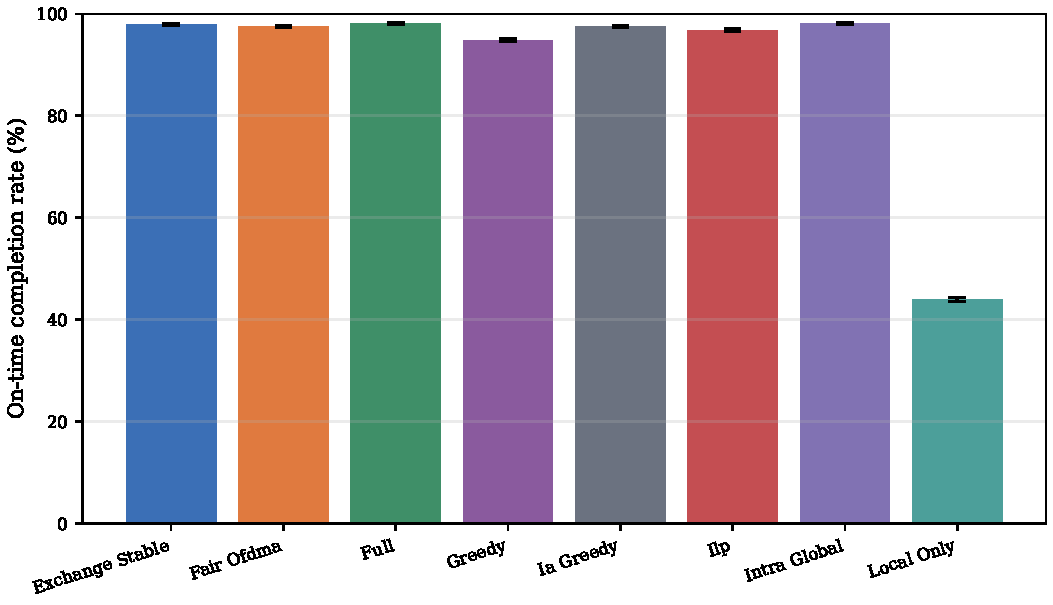
\includegraphics[width=0.9\textwidth]{../figures/thesis/main_on_time.pdf}
\caption{正式主实验按时完成率与确定性 bootstrap 区间}
\end{figure}
\begin{figure}[htbp]
\centering
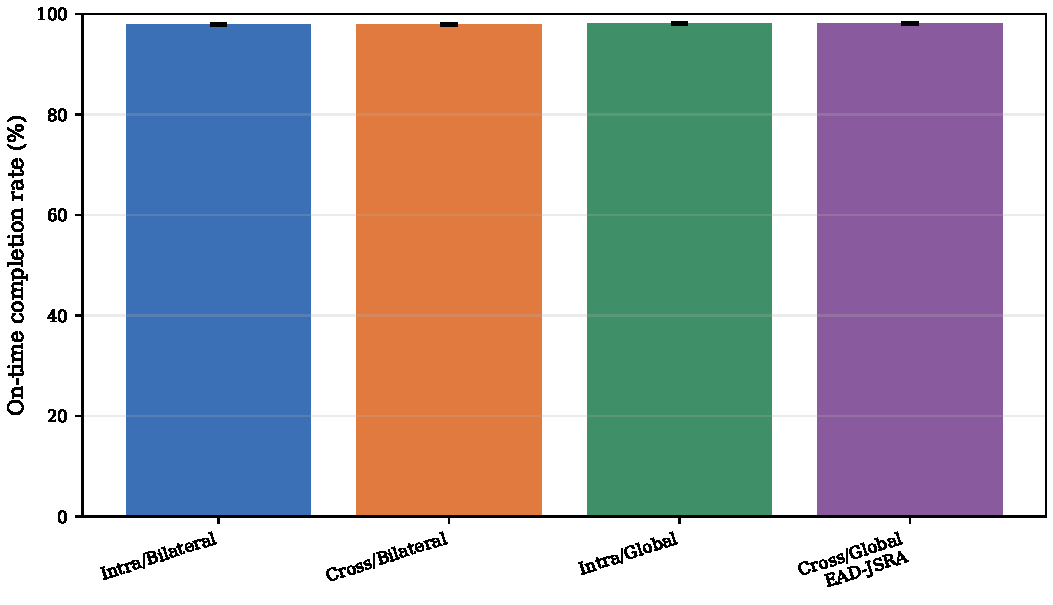
\includegraphics[width=0.78\textwidth]{../figures/thesis/pairing_ablation.pdf}
\caption{创新点一的拓扑与接受准则消融}
\end{figure}
\begin{figure}[htbp]
\centering
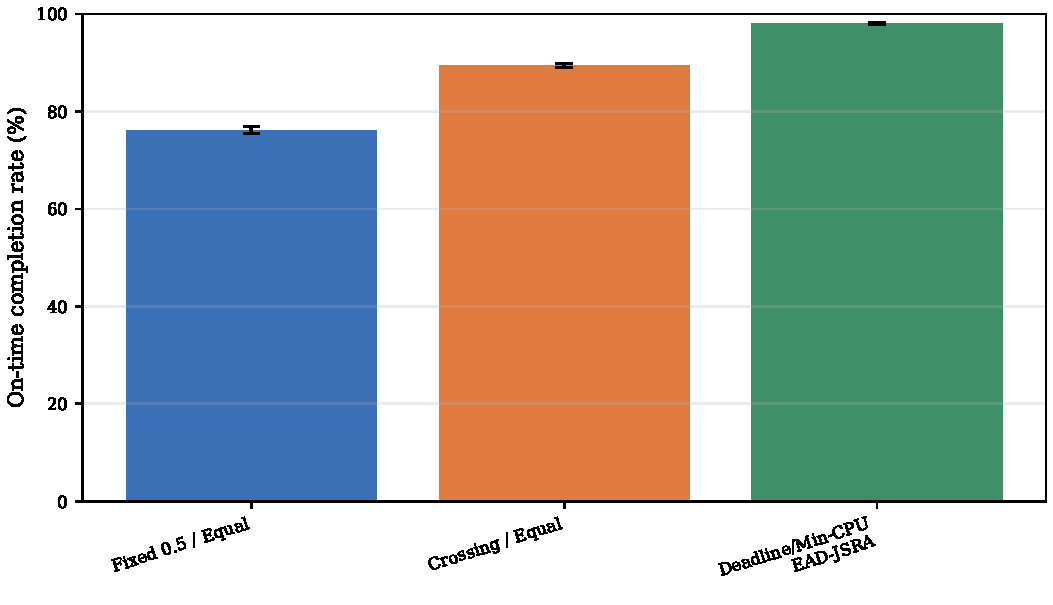
\includegraphics[width=0.78\textwidth]{../figures/thesis/resource_ablation.pdf}
\caption{创新点二的资源策略消融}
\end{figure}

\section{最优性、效率与鲁棒性}
小实例完整枚举中，启发式达到最优完成数的时隙比例为 \ExactOptimalPercent{}，平均完成数差距为 \ExactMeanCompletionGap{}；该结果仅覆盖冻结的小搜索空间。$N=20$ 的调度 P95 为 \FullRuntimePNinetyFiveMs{} ms。最终调度 SIC 违规计数为 \SICViolationCount{}。

随 $N$ 增长，所有方法按时率下降，full 在 $N=10\ldots50$ 均略高于 exchange-stable；随 $K$ 增长性能趋于饱和。$K=1$ 时 full 略低于 exchange-stable，$K=5$ 时二者持平，故不作全范围严格占优主张。轻负载下三方法均达到 100\%，重负载下 full 仍保持相对优势。

\begin{table}[htbp]
\centering
\caption{正式配对统计与主工程指标}
\resizebox{\textwidth}{!}{\begin{tabular}{lrrrr}
\toprule
Comparison & $\Delta$ (pp) & 95\% CI & $p_{\mathrm{Holm}}$ & $r_{rb}$ \\
\midrule
baseline\_exchange & 0.19 & [0.13, 0.26] & $<0.0001$ & 0.869 \\
baseline\_greedy & 3.24 & [2.96, 3.52] & $<0.0001$ & 1.000 \\
baseline\_ia\_greedy & 0.49 & [0.40, 0.59] & $<0.0001$ & 0.984 \\
baseline\_ilp & 1.30 & [1.16, 1.43] & $<0.0001$ & 1.000 \\
baseline\_ofdma & 0.58 & [0.45, 0.72] & $<0.0001$ & 0.950 \\
innovation1\_acceptance & 0.12 & [0.07, 0.16] & 0.0004 & 0.709 \\
innovation1\_cross & 0.05 & [0.01, 0.08] & 0.0201 & 0.521 \\
innovation2\_deadline & 8.69 & [8.37, 9.01] & $<0.0001$ & 1.000 \\
resource\_fixed\_half & 21.97 & [21.36, 22.60] & $<0.0001$ & 1.000 \\
\bottomrule
\end{tabular}

\bigskip

\begin{tabular}{lrrrrrr}
\toprule
Method & On-time (\%) & Drop (\%) & Delay (s) & Jain & CPU (\%) & P95 (ms) \\
\midrule
exchange\_stable & 97.91 & 2.09 & 0.6841 & 0.9993 & 33.58 & 30.14 \\
fair\_ofdma & 97.52 & 2.48 & 0.6837 & 0.9986 & 31.61 & 0.63 \\
full & 98.11 & 1.89 & 0.6843 & 0.9994 & 34.33 & 40.93 \\
greedy & 94.86 & 5.14 & 0.6804 & 0.9937 & 32.41 & 0.82 \\
ia\_greedy & 97.61 & 2.39 & 0.6838 & 0.9991 & 36.61 & 10.40 \\
ilp & 96.81 & 3.19 & 0.6828 & 0.9984 & 32.20 & 24.26 \\
intra\_global & 98.06 & 1.94 & 0.6843 & 0.9994 & 33.88 & 32.53 \\
local\_only & 43.94 & 56.06 & 0.5417 & 0.9707 & 0.00 & 0.19 \\
\bottomrule
\end{tabular}
}
\end{table}
